%\documentclass[a4paper,twoside,11pt]{article}
\documentclass[11pt, a4paper, oneside]{book} 
\usepackage[utf8]{inputenc}

\usepackage{amsmath,amssymb,amsthm}
\usepackage{mathtools}

%\usepackage[style=authoryear]{biblatex}
\usepackage[citestyle=authoryear,bibstyle=authoryear,natbib]{biblatex}
\addbibresource{Sources.bib}

\usepackage{caption}
\usepackage{subcaption}
\usepackage{float}
\usepackage{array}
\usepackage{graphicx}
\usepackage{pgfplots}
\pgfplotsset{compat=1.14}
\usepackage{tikz}
\usetikzlibrary{arrows,patterns,calc,matrix}

\usepackage[margin=1in]{geometry}
\usepackage{placeins}
\usepackage{flafter}
\usepackage[doublespacing]{setspace}

\usepackage{lipsum}
\usepackage{titlesec}
\usepackage{nomencl}
\makenomenclature
\usepackage[toc,page]{appendix}
\usepackage{verbatim}
%\usepackage{algorithm2e}
%\usepackage[noend]{algpseudocode}
\usepackage{xcolor}
\usepackage[cache=false]{minted}
\usepackage{listings}
\lstdefinestyle{lua}{
    language=[5.1]Lua,
    basicstyle=\ttfamily,
    tabsize=3,
    showspaces=false,
    showstringspaces=false,
    numbers=left,
    numberstyle=\color{lightgray},
    numbersep=5pt,
    %backgroundcolor=\color{black!5},
    keywordstyle=\color{teal},
    stringstyle=\color{red},
    commentstyle=\color{black!50}
}
\usepackage{import}

\usepackage{booktabs}
\usepackage{fancyhdr}

%\usepackage{cleveref}
\usepackage{hyperref}

%\title{Agent Based Modelling of Crowd Dynamics}
%\author{Alexander James Johnson}

% headers and footers
\pagestyle{fancy}
\setlength{\headheight}{14pt}
\renewcommand{\chaptermark}[1]{\markboth{\chaptername\ \thechapter.\ #1}{}}
\renewcommand{\sectionmark}[1]{\markright{\thesection.\ #1}}
\lhead{\rightmark}
\rhead{\leftmark}

\newcommand{\numberthis}{\addtocounter{equation}{1}\tag{\theequation}}
%\newcommand{\nr}[1]{\refstepcounter{equation}\label{#1}\tag{\theequation}}

\newcommand{\Rmag}[1]{\left|#1\right|}
\newcommand{\Rvec}[1]{\mathbf{#1}}
\newcommand{\Rnvec}[1]{\Rvec{\hat{#1}}}
\newcommand{\Rmvec}[1]{\Rmag{\Rvec{#1}}}
\newcommand{\Rtvec}[1]{\overset{\tau}{\Rvec{#1}}}
\newcommand{\Rntvec}[1]{\overset{\tau}{\Rnvec{#1}}}
\newcommand{\Rdt}{\ensuremath{\delta t}}
\newcommand{\Rovercast}[2]{\overset{\mathclap{\scriptscriptstyle#2}}{#1}}
\newcommand{\Rclamp}[1]{\ensuremath{\text{clamp}\left(#1\right)}}
\newcommand{\Rthresh}[2]{\ensuremath{\left\rmoustache#1\right\lmoustache_{#2}}}
\newcommand{\Rraisemath}[2]{\raisebox{#1}{$\displaystyle#2$}}
\newcommand{\Reg}{{\itshape e.g.~}}
\newcommand{\Rarrowscale}{0.5pt}

\newcommand{\HIDE}[1]{\PackageWarning{HIDE}{Hidden text in \thesubsection}}
\newcommand{\TODO}[1]{\texttt{TODO}: #1\PackageWarning{TODO}{#1}}


% intro to neural networks (background/history)
% - biological
% - artificial intelligence
% - preceptron
% - backpropagation
% - other types of networks
%   - convolutional
%   - recurrent
% introduction to python
% - neural networks in python
%   - single layer boston
%   - multilayer boston
%   - xor
% - tensorflow and keras
%   - boston
%   - xor
%   - linear regression
%   - character regression
% <application>
% - prior work
% - application aims
% - mathematics
% - neural network
% - results
% conclusion

\begin{document}

\begin{titlepage}
\begin{center}
    \vspace{2cm}
    \includegraphics[width = 6cm]{MMU_Logo_Colour.pdf}\\
    \textbf{\Large Faculty of Science and Engineering}\\
    \vspace{2cm}
    \textbf{\LARGE Alexander J. Johnson}\\
    \vspace{1cm}
    {\Large Mathematics}\\
    \vspace{1cm}
    \textbf{\LARGE Neural Networks with Python and TensorFlow}\\
    \vspace{1cm}
    {\Large\today}\\
    
    \vfill
    
    {\large School of Computing, Mathematics and Digital Technology}
\end{center}
\end{titlepage}

\addcontentsline{toc}{chapter}{Abstract}
\chapter*{Abstract}

Artificial Intelligence (AI) still remains as one of the greatest challenges in
scientific research to this date, but much progress in the field has been made
using artificial neural networks.
The design of artificial neural networks is loosely inspired by that of
biological brains, and serves as an expansion of an earlier concept called the
perceptron \citep{Rosenblatt:1958:Perceptron}.
By using multiple layers of these artificial neurons, we can form a highly
connected system that is referred to as a neural network,
these networks can then be trained on a large data set to predict the output
with high accuracy.

The range applications for neural networks is wide: they can be used to classify
data, predict future states of chaotic systems, apply stylisations to images,
or control physical/physically-based systems in real-time.

This project aims to cover the history of a wide range of artificial neural
networks and their applications.

\chapter*{Declaration}
With the exception of any statement to the contrary, all the material presented in this report is the result of my own efforts. In addition, no parts of this report are copied from other sources. I understand that any evidence of plagiarism and/or the use of unacknowledged third party materials will be dealt with as a serious matter.
\vspace{2cm}

Signed\vspace{-12pt}
\begin{center}
    \includegraphics[width=150pt]{Signiture.jpg}\vspace{-25.6pt}\\
	\line(1,0){250}
\end{center}
\tableofcontents
\chapter{Introduction to Neural Networks}

\TODO{Chapter: Introduction}

\section{Biological Neurons}

Biological neurons are electrically excitable cells that are found in almost all
animals.
These neurons can transmit and receive electrical signals to one another via
synaptic connections, which maybe either excitatory or inhibitory.
Any given neuron will be either active or inactive depending on whether or not
its input exceeds a threshold.

\begin{center}
    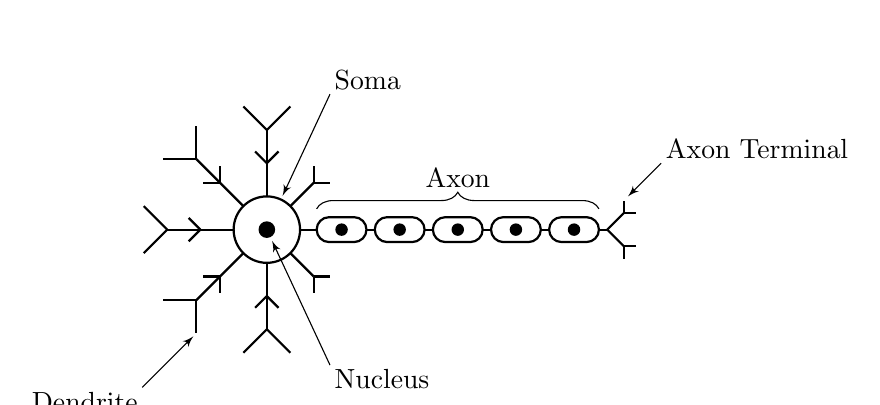
\begin{tikzpicture}%[x=1pt,y=1pt]
    \newlength{\rs}
    \setlength{\rs}{1.5pt}
    % Nucleus
    \fill (0\rs,0\rs) circle (2\rs);
    % Soma
    \draw[thick] (0\rs,0\rs) circle (8\rs);
    % Dendrite
    \draw[thick] ( 45:8\rs) -- ( 45:16\rs);
        \draw[thick] ( 45:16\rs) -- ++(  0:4\rs);
        \draw[thick] ( 45:16\rs) -- ++( 90:4\rs);
    \draw[thick] ( 90:8\rs) -- ( 90:24\rs);
        \draw[thick] ( 90:16\rs) -- ++( 45:4\rs);
        \draw[thick] ( 90:16\rs) -- ++(135:4\rs);
        \draw[thick] ( 90:24\rs) -- ++( 45:8\rs);
        \draw[thick] ( 90:24\rs) -- ++(135:8\rs);
    \draw[thick] (135:8\rs) -- (135:24\rs);
        \draw[thick] (135:16\rs) -- ++( 90:4\rs);
        \draw[thick] (135:16\rs) -- ++(180:4\rs);
        \draw[thick] (135:24\rs) -- ++( 90:8\rs);
        \draw[thick] (135:24\rs) -- ++(180:8\rs);
    \draw[thick] (180:8\rs) -- (180:24\rs);
        \draw[thick] (180:16\rs) -- ++(135:4\rs);
        \draw[thick] (180:16\rs) -- ++(225:4\rs);
        \draw[thick] (180:24\rs) -- ++(135:8\rs);
        \draw[thick] (180:24\rs) -- ++(225:8\rs);
    \draw[thick] (225:8\rs) -- (225:24\rs);
        \draw[thick] (225:16\rs) -- ++(180:4\rs);
        \draw[thick] (225:16\rs) -- ++(270:4\rs);
        \draw[thick] (225:24\rs) -- ++(180:8\rs);
        \draw[thick] (225:24\rs) -- ++(270:8\rs);
    \draw[thick] (270:8\rs) -- (270:24\rs);
        \draw[thick] (270:16\rs) -- ++(225:4\rs);
        \draw[thick] (270:16\rs) -- ++(315:4\rs);
        \draw[thick] (270:24\rs) -- ++(225:8\rs);
        \draw[thick] (270:24\rs) -- ++(315:8\rs);
    \draw[thick] (315:8\rs) -- (315:16\rs);
        \draw[thick] (315:16\rs) -- ++(270:4\rs);
        \draw[thick] (315:16\rs) -- ++(360:4\rs);
    % Axon
    \draw[thick] (8\rs,0\rs) -- (12\rs,0\rs);
    \draw[thick,rounded corners=3\rs] (12\rs,-3\rs) rectangle (24\rs,3\rs);
        \fill (18\rs,0\rs) circle (1.5\rs);
    \draw[thick] (24\rs,0\rs) -- (26\rs,0\rs);
    \draw[thick,rounded corners=3\rs] (26\rs,-3\rs) rectangle (38\rs,3\rs);
        \fill (32\rs,0\rs) circle (1.5\rs);
    \draw[thick] (38\rs,0\rs) -- (40\rs,0\rs);
    \draw[thick,rounded corners=3\rs] (40\rs,-3\rs) rectangle (52\rs,3\rs);
        \fill (46\rs,0\rs) circle (1.5\rs);
    \draw[thick] (52\rs,0\rs) -- (54\rs,0\rs);
    \draw[thick,rounded corners=3\rs] (54\rs,-3\rs) rectangle (66\rs,3\rs);
        \fill (60\rs,0\rs) circle (1.5\rs);
    \draw[thick] (66\rs,0\rs) -- (68\rs,0\rs);
    \draw[thick,rounded corners=3\rs] (68\rs,-3\rs) rectangle (80\rs,3\rs);
        \fill (74\rs,0\rs) circle (1.5\rs);
    % Axon terminal
    \draw[thick] (80\rs,0\rs) -- (82\rs,0\rs);
        \draw[thick] (82\rs,0\rs) -- (86\rs,4\rs);
            \draw[thick] (86\rs,4\rs) -- (86\rs,7\rs);
            \draw[thick] (86\rs,4\rs) -- (89\rs,4\rs);
        \draw[thick] (82\rs,0\rs) -- (86\rs,-4\rs);
            \draw[thick] (86\rs,-4\rs) -- (86\rs,-7\rs);
            \draw[thick] (86\rs,-4\rs) -- (89\rs,-4\rs);
    % Labels
    % Soma
    \draw[latex'-] (65:9\rs) -- (65:36\rs);
    \node[anchor=south west,inner sep=1\rs] at (65:36\rs) {Soma};
    % Nucleus
    \draw[latex'-] (-65:3\rs) -- (-65:36\rs);
    \node[anchor=north west,inner sep=1\rs] at (-65:36\rs) {Nucleus};
    % Dendrite
    %\draw[latex'-] (225:25\rs) -- (225:36\rs);
    \draw[latex'-] (-17.7\rs,-25.7\rs) -- (-30\rs,-38\rs);
    \node[anchor=north east,inner sep=1\rs] at (-30\rs,-38\rs) {Dendrite};
    % Axon
    \draw[decorate,decoration={brace,raise=5\rs,amplitude=4\rs}] (12\rs,0\rs) -- (80\rs,0\rs);
    \node[anchor=south,inner sep=1\rs] at (46\rs,9\rs) {Axon};
    % Axon Terminal
    \draw[latex'-] (87\rs,8\rs) -- (95\rs,16\rs);
    \node[anchor=south west,inner sep=1\rs] at (95\rs,16\rs) {Axon Terminal};
\end{tikzpicture}

    \captionof{figure}{Diagram of a biological neuron.}
\end{center}

Signals are received by the neuron via connections to dendrites and soma.
If the threshold is met, electrical signals are sent along the axon to the
terminal, where it is connected to other neurons, or to a controllable cell such
as a neuromuscular junction.

\TODO{Section: Biological Neurons}

\section{Artificial Intelligence}

The idea of artificial beings capable of human intelligence can be traced back
to mythical stories from ancient Greece.
One such story was that of a mythical automaton called Talos, who circled an
island's shores to protect it from pirates and other invaders.

By the $19^\text{th}$ century, other notions of artificial intelligence were
explored by fiction in stories such as Mary Shelley's ``Frankenstein'', and
Karel \v{C}apek's ``R.U.R.''.
Some of the fictional writings of the $20^\text{th}$ century further continued
exploring the concept in novels such as Isaac Asimov's ``I, Robot''.

Academic research into artificial intelligence began around the 1940's,
primarily due to findings in neurological research at the time.
The first explorations of artificial neural networks was done by
\cite{McCulloch:1943:Logical}, who investigated how simple logic functions
might be performed by idealised networks.
The neurons within these networks operated using some basic logic rules, applied
to a discrete time system which, can be summarised using the expression
\begin{align*}
    N(t) &= (E_1(t-1) \vee E_2(t-1) \vee \dots)
        \wedge \neg(I_1(t-1) \vee I_2(t-1) \vee \dots),
\end{align*}
where $N(t)$ is the state of a neuron at time $t$, and $E_i(t-1)$ and $I_i(t-1)$
are the states of the excitatory and inhibitory connections from the previous
time step respectively.
The result is such that the neuron will only be active if at least one
excitatory connection is active and all inhibitory connections are inactive.
The versatility of this definition is demonstrated in the following examples.
\begin{center}
    \begin{tabular}{ccc}
        SR Flip-flop & & AND Gate\\
        \begin{tikzpicture}
    [   neuron/.style=
        {   draw
        ,   regular polygon
        ,   regular polygon sides=3
        ,   shape border rotate=90
        ,   inner sep=2pt
        ,   node font=\small\ttfamily
        }
    ,   baseline=0pt
    ]
    \node[neuron] (S) at (0cm, 7mm) {S};
    \node[neuron] (R) at (0cm,-7mm) {R};
    \node[neuron] (M) at (2cm, 0cm) {M};
    \draw[arrows={-Rrrow}] (S) to[out=0,in=150] (M);
    \draw[-Circle] (R) to[out=0,in=210] (M);
    \draw[-latex'] (M.east) .. controls (3cm,1cm) and (2cm,1cm) .. (M);
    \draw[-latex'] (M.east) to (3cm,0cm);
\end{tikzpicture}
 & & \begin{tikzpicture}
    [   neuron/.style=
        {   draw
        ,   regular polygon
        ,   regular polygon sides = 3
        ,   shape border rotate = 90
        ,   inner sep = 2pt
        ,   node font = \small\ttfamily
        }
    ,   baseline = 0pt
    ,   > = {Stealth[scale=1.2]}
    ]
    \node[neuron] (A) at (-2cm, 6mm) {A};
    \node[neuron] (B) at (-2cm,-6mm) {B};
    \node[neuron] (Af) at (0cm, 18mm) {1};
    \node[neuron] (Ab) at (0cm,  6mm) {2};
    \node[neuron] (Ba) at (0cm, -6mm) {3};
    \node[neuron] (Bf) at (0cm,-18mm) {4};
    \node[neuron] (R) at (2cm,0cm) {R};
    \draw[->] (A) to[out=0,in=240] (Af);
    \draw[->] (B) to[out=0,in=120] (Bf);
    \draw[->] (Af) to[out=0,in=120] (R);
    \draw[->] (Bf) to[out=0,in=240] (R);
    \draw[->] (A) to[out=0,in=120] (Ba);
    \draw[->] (B) to[out=0,in=240] (Ab);
    \draw[-o] (A) to[out=0,in=180] (Ab);
    \draw[-o] (B) to[out=0,in=180] (Ba);
    \draw[-o] (Ab) to[out=0,in=180] (R.west);
    \draw[-o] (Ba) to[out=0,in=180] (R.west);
\end{tikzpicture}
\\
        $\displaystyle N_M(t+1) = (N_S(t) \vee N_M(t)) \wedge\neg N_R(t)$ &
        &
        $\displaystyle N_R(t+2) = N_A(t) \vee N_B(t)$\\
    \end{tabular}
    \parbox{0.9\textwidth}{%
    \captionof{figure}{Two common logic circuits using McCullochs neurons
    where the arrows and circles indicate excitatory and inhibitory
    connections respectively.}}
\end{center}
While this model provided insight into the mechanisms by which neurons operate,
the structure was static, and incapable of learning.

McCulloch's work was later cited by psychologist \cite{Hebb:1949:Organization},
who proposed that the structure of biological neural networks was dynamic, and
that frequently repeated stimuli caused gradual development.
At the scale of neuron, it was theorised that if one neuron successfully
excited another that the connection between them would strengthen, hence
increasing the likelihood that the former would be able to excite the latter
again in the future.
His theory was supported by research conducted by himself and others that showed
that intelligence-test performance in mature patients was often unaffected by
brain operations that would have prevented development in younger patients,
which suggested that learnt stimuli are processed differently to unknown
stimuli.
This hypothesis became known as Hebbian learning.

Computer simulations applying this theory to a small network were done by
\cite{Farley:1954:Simulation}.
The actions of the network were compared to that of a servo system which must
counteract any displacements so as to maintain a steady position.
The network was trained using a set of input patterns, which were subject to
non-linear transformations.
Similar to the Hebbian theory, when the network produces the correct responses,
the active connections are strengthened.
Although the results were of little neurophysiological significance, the results
were of great use for demonstrating computational simulations, which were
considerably slower at the time.

\TODO{Section: Artificial Intelligence}

\subsection{Perceptrons}

The idea of the perceptron was originally conceived by
\cite{Rosenblatt:1958:Perceptron}, to represent a simplified model of
intelligent systems free from particularities of biological organisms, whilst
maintaining some of their fundamental properties.

The perceptron was built as a dedicated machine that consisted of a number of
photovoltaic cells, analogous to a retina, that feed into an``association
area''.
This association area contains a number of cells that each calculate a weighted
sum of the receptor values and output a signal if it exceeds a threshold.
Expressed mathematically, the output of a given association cell is given by
\begin{align*}
    A_i &= \begin{cases}
        1, & \sum_j w_{i,j}x_j\\
        0, & \text{otherwise}
    \end{cases},
\end{align*}
where $x_j$ is the value from the $j^\text{th}$ photovoltaic cell, and $w_{i,j}$
is the weight there of.
These value weights were implemented using variable resistance wires that the
perceptron could adjust automatically.
The outputs from the association area are then connected to response cells,
which operate in a similar fashion to the association cells.
The activation of these response cells are the outputs of the perceptron, and
indicated the classification of the input.

Similar to \cite{Farley:1954:Simulation}, the method by which the perceptron
adjusted it weights was also based on which cells were active, and whether the
correct output was produced; except that the perceptron was also able to
``penalise'' weights when an incorrect result was outputted.

This machine was initially trained to reliably identify three different shapes:
a square, a circle, and a triangle; and did so with a better than chance
probability.
When attempting to use the perceptron for more complicated tasks, such as
character recognition, it failed to produce better than chance results.

\TODO{Subsection: Perceptrons}

\subsection{Backpropagation}

In order for a neural network to learn, it must undergo some form of
optimisation process.
For the perceptron, this process was one of positive and negative reinforcement.

In the field of control theory, an optimisation method known as gradient descent
was developed by \cite{Kelley:1960:Gradient}, in which a given function of the
system is either maximised or minimised.
This is achieved by taking partial derivatives of the function with respect to
each parameter, which gives an approximation of how the function value will
change as the parameter changes.
By evaluating the partial derivatives, multiplying them by a constant, and
adding them to their respective parameters, the parameter values can be updated.
Using these new parameter values, one can expect to improve the function value.
This can be written as
\begin{align*}
    w_i' &= w_i + \eta\Rpdiff{f}{w_i}(\Rvec{x}),
\end{align*}
where $f(\Rvec{x})$ is the function to be optimised, $w_i$ is a parameter of
$f$, $w_i'$ is the updated parameter, and $\eta$ is ascent/descent parameter.
Positive $\eta$ values will maximise the function value, where as negative
values will minimise it.
The magnitude of $\eta$ determines the rate at which the method will attempt
change the parameters: if the value is too large, the method will overshoot the
optimal values; if the value is too small, the method will be too slow to
converge.

\TODO{Subsection: Backpropagation}

\section{Types of Neurons}

\TODO{Section: Types of Neurons}

\subsection{CNN}
\subsection{RNN}
\subsection{LSTM}

\chapter{Introduction to Python}

Python is a general-purpose programming language designed by Guido van Rossum,
with an emphasis on readability and reusability \citep{vanRossum:1996:Foreword}.
It comes with an extensive standard library and is one of the most popular
programming languages.

There are multiple options for interacting with Python, these include:
\begin{itemize}
    \item typing commands into an interpreter,
    \item writing files and running them with an interpreter,
    \item using an online service such as Google Colab.
\end{itemize}
A small snippet of trivial python code is given below to display the syntax.
{\singlespacing
\inputminted[
    frame=lines,
    framesep=2mm,
    mathescape,
    linenos
    ]{python}{Sample.py}
}

\section{Neural Networks in Python}

Before using any neural network packages, a few small examples networks were
produced in python.
The \texttt{numpy} package was used to perform matrix operations,
and the \texttt{matplotlib.pyplot} package was used for plotting,
as these features were non-trivial.
For some examples, the \texttt{keras} module from the \texttt{tensorflow}
package was also used to access specific datasets, but their broader purpose
will be explored in the next section.

\subsection{Single Layer Boston Housing Data}

The first example network consisted of 3 input neurons connected to a
single output neuron, which is given by the equation
\begin{align*}
    y &= \tanh\left(b + \sum_{i=1}^{3} w_ix_i\right).
\end{align*}
The bias term was implemented by adding a forth input node with a constant value
of one, giving
\begin{align*}
    y &= \tanh\left(\mathbf{w}\cdot\mathbf{x}\right),
\end{align*}
where $w_4 = b$, and $x_4 = 1$.

The network was trained using the Boston housing dataset from \texttt{keras},
which provided a number of attributes about houses from late 1970's Boston
suburbs.
The network took in normalised data from three of these attributes (number of
rooms, highway accessibility index, percentage of lower status population), and
used them to predict the value of the house.

Training was performed using backpropagation, defined by the equation
\begin{align*}
    \Delta w_i &= \eta\Rpdiff{e}{w_i},\\
    d &= y - y_t,\\
    e &= \frac{1}{2}d^2,
\end{align*}
where $e$ is the network error, $y$ is the network prediction, and $y_t$ is the
target value.
By definition,
\begin{align*}
    y &= \tanh(\text{net}),\\
    \text{net} &= \sum w_ix_i.
\end{align*}
By chain rule,
\begin{align*}
    \Rpdiff{e}{w_i} &=
    \Rpdiff{e}{y} \cdot \Rpdiff{y}{\text{net}} \cdot \Rpdiff{\text{net}}{w_i}.\\
    %
    \Rpdiff{net}{w_i} &= x_i,\\
    \Rpdiff{y}{net} &= 1 - \tanh^2(net) = 1 - y^2,\\
    \Rpdiff{e}{y} &= \frac{1}{2}\Rpdiff{(y - y_t)^2}{y} = y - y_t = d,\\
    %
    \therefore\Rpdiff{e}{w_i} &=
    x_i \cdot (1 - y^2) \cdot d.
\end{align*}
$\Delta w_i$ can be written in vector notation, giving
\begin{align*}
    \Delta \mathbf{w} &= \eta\cdot\mathbf{x}\cdot (1-y^2)\cdot d.
\end{align*}
Weights were updated after each sample using
\begin{align*}
    \mathbf{w}' &= \mathbf{w} - \Delta\mathbf{w},
\end{align*}
where $\mathbf{w}'$ is the new set of weights.

The network was initialised using random weights, and was trained using the full
dataset.
\rfig{\begin{tikzpicture}
    \begin{axis}
        [   width = 0.8\textwidth
        ,   xtick = {0,1000,2000,3000,4000,5000}
        ,   legend pos = south west
        ,   xlabel = {Iteration}
        ,   ylabel = {Value}
        ]
        \addplot [color = Rblue]   table [col sep = comma]
        {../Code/BostonHousing/DataPythonSingleW0.csv};
        \addplot [color = Rorange] table [col sep = comma]
        {../Code/BostonHousing/DataPythonSingleW1.csv};
        \addplot [color = Rgreen]  table [col sep = comma]
        {../Code/BostonHousing/DataPythonSingleW2.csv};
        \addplot [color = Rred]    table [col sep = comma]
        {../Code/BostonHousing/DataPythonSingleW3.csv};
        \legend{$w_0$,$w_1$,$w_2$,$w_3$}

        \addplot
        [   opacity = 0.2
        ,   sharp plot
        ,   update limits = false
        ]   coordinates {(0,-1) (0,1)};
        \pgfplotsinvokeforeach{1,...,10}%
        {   \addplot
            [   opacity = 0.2
            ,   sharp plot
            ,   update limits = false
            ]   coordinates {(506*#1,-1) (506*#1,1)}
            node [anchor = south, rotate = 90] at (506*#1,0.05) {\tiny epoch = #1};
        }
    \end{axis}
\end{tikzpicture}
}{%
    Graph of network weights against iteration number.
}
After 10 epochs, the mean square error had reduced from 0.1637 to 0.0507.
Note that the weight value lines appear to be jagged, this was a side effect of
updating the value after each individual presentation; a problem which can be
mitigated by batching $\Delta\mathbf{w}$ terms from multiple presentations.



\subsection{Multilayer Boston Housing Data}

The same task was repeated using the full set of attributes.
To accommodate this, a larger network with 13 input neurons, 1 output neuron,
and $n$ hidden neurons; which was expressed by the equation
\begin{align*}
    h_i &= \tanh\left(b_i + \sum_{j=0}^{13} w_{i,j}x_j\right),\\
    y &= b + \sum_{i=1}^{n} w_i h_i.
\end{align*}
Similar to the single layer example, a constant neuron was added to the input
and hidden layer to implement the bias, giving
\begin{align*}
    \mathbf{h} &= \tanh(W\mathbf{x}),\\
    \mathbf{h}' &= \begin{pmatrix} \mathbf{h} \\ 1 \end{pmatrix},\\
    y &= \mathbf{w}\cdot\mathbf{h}',
\end{align*}
where $\tanh$ acts component-wise on the input.

All of the inputs were batched together into a single matrix $X$, where each
column was a data point, giving
\begin{align*}
    \Phi &= \tanh(W\cdot X),\\
    \Psi &= \begin{pmatrix} \Phi \\ \mathbf{1} \end{pmatrix},\\
    \mathbf{y} &= \mathbf{w}\cdot\Psi,
\end{align*}
where $\mathbf{y}$ is a row vector of results.
The error gradients for the output neurons were given by
\begin{align*}
    \mathbf{d} &= \mathbf{y} - \mathbf{y}_t,\\
    e &= \frac{1}{2}\left|\mathbf{d}\right|^2,\\
    \mathbf{g}_O &= \Rpdiff{e}{\mathbf{w}} = \mathbf{d}\cdot\Psi^T;
\end{align*}
and for the hidden neurons by
\begin{align*}
    D &= \hat{\mathbf{w}}^T\cdot\mathbf{d},\\
    G_H &= ((1 - \Phi\odot\Phi)\odot D) \cdot X^T,
\end{align*}
where $\odot$ is the component-wise product, and $\hat{\mathbf{w}}$ is the
weight vector without the bias term.
Note that $\hat{\mathbf{w}}^T$ and $\mathbf{e}$ are column and row vectors
respectively, and that their product is a matrix.
See Appendix \ref{app:BHMDeriv} for full derivation.
\rfig{\begin{tikzpicture}
    \begin{axis}
        [   width = 0.8\textwidth
        ,   xtick = {0,100,200,300,400,500}
        ,   legend pos = north east
        ,   xlabel = {Epoch}
        ,   ylabel = {Loss}
        ]
        \addplot [color = Rblue]   table [col sep = comma]
        {../Code/BostonHousing/DataPythonMulti1.csv};
        \addplot [color = Rorange] table [col sep = comma]
        {../Code/BostonHousing/DataPythonMulti2.csv};
        \addplot [color = Rgreen]  table [col sep = comma]
        {../Code/BostonHousing/DataPythonMulti3.csv};
        \legend{Hidden = 1,Hidden = 2,Hidden = 3}
    \end{axis}
\end{tikzpicture}
}{%
    Graph of network error against iteration number for
    various numbers of hidden neurons using the Boston housing data.
}
The network was trained multiple times with varying numbers of hidden neurons.
The same random seed value was used for all trials.
In each case, the network successfully reduced it's error to roughly the same
level:
for 1 neuron, from 0.1670 to 0.0380;
for 2 neurons, from 0.1799 to 0.0390; and
for 3 neurons, from 0.1757 to 0.0396.
The difference between the results was negligible, which suggested that one
hidden neuron was sufficient for learning the data.

When compared with the single layer network from the previous section, the
single neuron, multilayer network performed better (0.0507 vs 0.0380) for two
reasons:
\begin{enumerate}
    \item it had access to all 13 attributes, instead of the 3 attributes that
        had been manually selected; and
    \item the additional layer enabled it to apply a linear transformation to
        the activation.
\end{enumerate}
Additionally, the use of batched inputs resulted in a smoother descent, as the
total gradient is descended; instead of multiple, often opposing gradients.



\subsection{Logical XOR}

Using the same, multilayer network architecture, a network was trained to
perform the logical exclusive-or (XOR) operation.
The input matrix $X$ contained all four combinations of binary inputs, and the
target outputs in $\mathbf{y}_t$.
\begin{align*}
    X &= \begin{pmatrix}
        0 & 1 & 0 & 1 \\
        0 & 0 & 1 & 1 \\
        1 & 1 & 1 & 1
    \end{pmatrix},\\
    \mathbf{y}_t &= \begin{pmatrix}
        0 & 1 & 1 & 0
    \end{pmatrix}.
\end{align*}
Given that the problem is mathematically well defined, a successfully trained
network should reduce the error to near zero.
Training the network for varying numbers of hidden neurons gave the following
results.
\rfig{\begin{tikzpicture}
    \begin{axis}
        [   width = 0.8\textwidth
        ,   xtick = {0,50,100,150,200,250,300}
        ,   legend pos = north east
        ,   xlabel = {Epoch}
        ,   ylabel = {Loss}
        ]
        \addplot [color = Rblue]   table [col sep = comma]
        {../Code/XOR/DataPython1.csv};
        \addplot [color = Rorange] table [col sep = comma]
        {../Code/XOR/DataPython2.csv};
        \addplot [color = Rgreen]  table [col sep = comma]
        {../Code/XOR/DataPython3.csv};
        \legend{Hidden = 1,Hidden = 2,Hidden = 3}
    \end{axis}
\end{tikzpicture}
}{%
    Graph of network error against iteration number for
    various numbers of hidden neurons using the XOR data.
}
The final mean square errors for one, two, and three hidden neurons were 0.1713,
$2.04\times10^{-5}$, and $9.65\times10^{-6}$ respectively.
These results showed that a single, nonlinear neuron is not sufficient for
learning the XOR problem, as proven by \cite{Minsky:1969:Perceptrons}, and is
only capable of solving three of the four inputs at a time.
Two nonlinear neurons is sufficient for solving the problem.

It is important to note that the learning rates were much more susceptible to
the initial weights than that of the Boston housing data.
Under certain initial conditions, the network displayed long periods of
negligible change before significant learning occurred, the longest of which
that had been observed lasted over 800 iterations.
Error spiking was observed across the majority of initial conditions for both
two and three hidden neurons.



\section{Using TensorFlow and Keras}

Creating efficient neural networks by hand was difficult, repetitive, and prone
to mistakes; and making simple modifications, such as changing the activation
function, could prove tricky for larger networks.
Thankfully, python packages that automate large portions of the process are
available, namely TensorFlow.

Once installed, TensorFlow can be imported into python.
TensorFlow contains a module called Keras, which provides a number of objects
and constructors that make the process much simpler.
The XOR network, for instance, can be constructed with a few lines of code.
\begin{minted}[
    frame=lines,
    framesep=2mm,
    mathescape,
    linenos
    ]{python}
import tensorflow as tf
layers = tf.keras.layers
# Create a model
model = tf.keras.models.Sequential()
# Add a dense hidden layer with the built in $\tanh$ activation function
model.add(layers.Dense(3, input_dim=2, activation='tanh')
# Add the output layer with linear activation
model.add(layers.Dense(1))
# Finalise the model and specify the loss function
model.compile(loss='mean_squared_error')
\end{minted}
TensorFlow provides multiple ways of constructing models, and a wide variety of
options to configure layers, models, and optimisers, as well as custom
definitions.

TensorFlow also supports multithreading and GPU acceleration, making it
especially suitable for large networks and training sets.



\subsection{Boston Housing}

The Boston housing example was repeated using TensorFlow, with two hidden
layers, each with five neurons using the $\tanh$ activation function, and a
linear output layer, to see if adding additional layers and neurons would
improve the results.
The data was also split into two groups, training and validation, the latter of
which was not used for training the network.
For a well-fitting network, the loss values for both groups should be similar,
and the ratio between them provided a rough measure of over-fitting.

The network was trained over 2000 epochs using the stochastic gradient descent
optimiser, obtaining an final training loss of 0.0421, and validation loss of
0.0396.
The ratio between the loss values is $\sim0.94$, this value is close to 1,
suggesting that the network was not over-fitting.
\rfig{\begin{tikzpicture}
    \begin{axis}
        [   width = 0.8\textwidth
        ,   xtick = {0,500,1000,1500,2000}
        ,   ymin = 0
        ,   legend pos = north east
        ,   xlabel = {Epoch}
        ,   ylabel = {Loss}
        ]
        \addplot [color = Rblue]   table [col sep = comma]
        {../Code/BostonHousing/DataTensorSGDLoss.csv};
        \addplot [color = Rorange] table [col sep = comma]
        {../Code/BostonHousing/DataTensorSGDVali.csv};
        \legend{Training,Validation}
    \end{axis}
\end{tikzpicture}
}{%
    Graph of training and validation loss against iteration
    number with ``SGD'' optimiser.
}
\newpage
The network was trained again using the ``Adam'' optimiser
\citep{Kingma:2014:Adam}, which uses estimations of both first and second-order
moments, and consistently outperforms the stochastic gradient descent method.

With the Adam optimiser, the final training and validation loss values were
0.0147 and 0.0443 respectively.
Although the loss value is smaller than with stochastic gradient descent, the
loss ratio was $\sim3.01$, which suggests that the network was over-fitting.
This was further evidenced the loss graph, which show that beyond a certain
point, the training loss and validation loss diverge, with the validation loss
increasing.
As such, the network is expected to be less generalised.
\rfig{\input{DiagramBHTFAdam.tex}}{%
    Graph of training and validation loss against iteration
    number with ``Adam'' optimiser.
}

%2000 epochs

%SGD [5,5]
%initial loss 0.228166446089744570
%  final loss 0.042430859059095380
%initial vali 0.214338675141334530
%  final vali 0.046398963779211044
% vali / loss 1.093519311

%SGD [3,3]
%initial loss 0.285416126251220700
%  final loss 0.033157549798488620
%initial vali 0.329692572355270400
%  final vali 0.045487113296985626
% vali / loss

%SGD [3]
%initial loss 0.494845181703567500
%  final loss 0.041440241038799286
%initial vali 0.568243682384491000
%  final vali 0.048694450408220290

%Adams [5,5]
%initial loss 0.425099462270736700
%  final loss 0.014745806343853474
%initial vali 0.409027785062789900
%  final vali 0.044336102902889250

\subsection{Linear Regression}

\rfig{\begin{tikzpicture}
    \pgfplotsset{
        % define the layers you need.
        % (Don't forget to add `main' somewhere in that list!!)
        layers/my layer set/.define layer set =
        {   bottom
        ,   main
        ,   top
        }{
            % you could state styles here which should be moved to
            % corresponding layers, but that is not necessary here.
            % That is why wo don't state anything here
        },
        % activate the newly created layer set
    }
    \begin{axis}
        [   width = 0.8\textwidth
        ,   legend pos = north west
        ,   xmin = -0.1
        ,   ymin = -0.1
        ,   xmax =  1.1
        ,   ymax =  1.1
        ,   xtick = {0,0.2,0.4,0.6,0.8,1}
        ,   ytick = {0,0.2,0.4,0.6,0.8,1}
        ,   xlabel = {$x$}
        ,   ylabel = {$y$}
        ,   set layers = my layer set
        ]
        \addplot [on layer = bottom, color = Rblue, only marks, mark size = 1pt]
        table [col sep = comma]
        {../Code/Regression/DataLinearPoints.csv};
        \addplot [on layer = top, color = Rorange]
        table [col sep = comma]
        {../Code/Regression/DataLinearPrediction.csv};
        \legend{Data,Prediction}
    \end{axis}
\end{tikzpicture}
}{%
    Graph showing the data points and network's corresponding line of best fit.
}
%initial loss 0.62278741598129270000
%  final loss 0.00022495193115901202

\subsection{Character Recognition}

\rfig{\begin{tikzpicture}
    \foreach\posx/\posy/\pred/\cert/\actu in
    {   0/0/7/1.00/7
    ,   1/0/2/1.00/2
    ,   2/0/1/0.99/1
    ,   3/0/0/1.00/0
    ,   4/0/4/0.99/4
    ,   0/1/1/0.99/1
    ,   1/1/4/0.99/4
    ,   2/1/9/0.97/9
    ,   3/1/6/0.82/5
    ,   4/1/9/0.98/9
    ,   0/2/0/1.00/0
    ,   1/2/6/1.00/6
    ,   2/2/9/1.00/9
    ,   3/2/0/1.00/0
    ,   4/2/1/1.00/1
    ,   0/3/5/0.99/5
    ,   1/3/9/0.99/9
    ,   2/3/7/1.00/7
    ,   3/3/3/0.91/3
    ,   4/3/4/1.00/4
    ,   0/4/9/0.98/9
    ,   1/4/6/0.99/6
    ,   2/4/6/1.00/6
    ,   3/4/5/1.00/5
    ,   4/4/4/0.98/4
    }
    {   \pgfmathtruncatemacro{\indx}{5*\posy+\posx}
        \node[draw] (N\indx) at (3*\posx,-3.8*\posy)
        {\includegraphics[width=1.5cm]{CRResults/img\indx}};
        %\node (T\indx) at (N\indx.north) [anchor=south]
        %    {\scriptsize Was: \actu};
        %\node (D\indx) at (N\indx.south) [anchor=north]
        %    {\scriptsize Predicted: \pred};
        %\node at (D\indx.south) [anchor=north,outer sep=0pt,inner sep=0pt]
        %    {\scriptsize (\cert)};
        \node (P\indx) at (N\indx.north) [anchor=south]
        {\scriptsize Predicted: \pred};
        \node (A\indx) at (P\indx.north) [anchor=south,outer sep=0,inner sep=0]
        {\scriptsize Was: \actu};
        \node (S\indx) at (N\indx.south) [anchor=north]
        {\scriptsize \ifnum \actu=\pred
                Correct
            \else
                \underline{\textbf{Incorrect}}
            \fi};
        \node (C\indx) at (S\indx.south) [anchor=north,outer sep=0,inner sep=0]
        {\scriptsize Certainty: \cert};
    }
\end{tikzpicture}
}{%
    Hand written numbers from the MNIST validation set, the network prediction,
    and the certainty of the network.
}
%500 epochs
%initial loss: 2.3656811714172363
%  final loss: 0.06899717450141907
%initial vali: 2.1969106197357178
%  final loss: 0.10314085334539413
%  training size:   60000
%validation size:   10000
%  training errors: 4223
%validation errors: 1247
%  training %err:   7.038333333333333
%validation %err:   12.47

%Convol: 50 epochs, batch=600
%initial loss: 0.5744658349454403
%initial vali: 0.2477983083575964
%final loss:   0.010112296480219812
%final loss:   0.05892044545849785
%training size:     60000
%training errors:   482
%training %err:     0.8033333333333333
%validation size:   10000
%validation errors: 493
%validation %err:   4.93


\chapter{Introduction To TensorFlow}

TensorFlow
\TODO{Chapter: Introduction To TensorFlow}

\section{Linear Regression}

\TODO{Section: Linear Regression}

\section{XOR}

\TODO{Section: XOR}

\section{Boston Housing with Keras}

\TODO{Section: Boston Housing with Keras}

\chapter{Deep Learning}

\TODO{Chapter: Deep Learning}

\section{Recurrent Neural Networks}

\TODO{Section: Recurrent Neural Networks}

\section{Convolutional Neural Networks}

\TODO{Section: Convolutional Neural Networks}

\subsection{Image Processing}

\TODO{Subsection: Image Processing}

\section{Supervised Learning}

\TODO{Section: Supervised Learning}

\section{Unsupervised Learning}

\TODO{Section: Unsupervised Learning}

\section{Autoencoding}

\TODO{Section: Autoencoding}

\section{Reinforcement Learning}

\TODO{Section: Reinforcement Learning}




\chapter{Null}

%\underline{\textbf{notes.txt}}
%{\singlespacing\lstinputlisting[basicstyle=\tiny]{../notes.txt}}
\HIDE{\begin{center}
    \captionof{figure}{Diagram of a biological neuron.}
    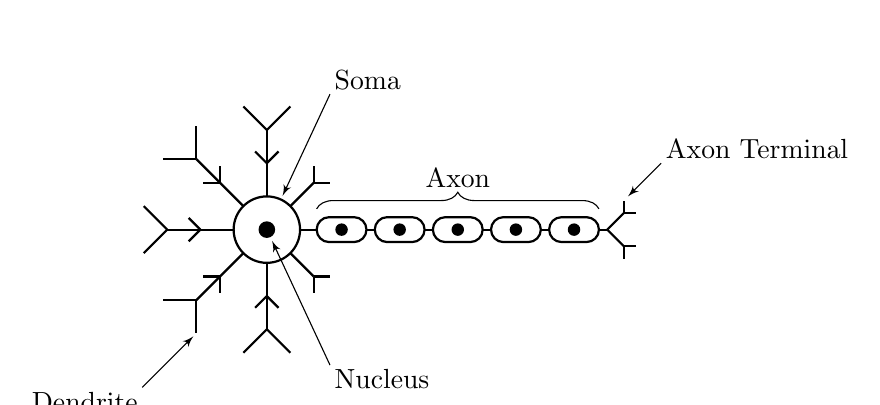
\begin{tikzpicture}%[x=1pt,y=1pt]
    \newlength{\rs}
    \setlength{\rs}{1.5pt}
    % Nucleus
    \fill (0\rs,0\rs) circle (2\rs);
    % Soma
    \draw[thick] (0\rs,0\rs) circle (8\rs);
    % Dendrite
    \draw[thick] ( 45:8\rs) -- ( 45:16\rs);
        \draw[thick] ( 45:16\rs) -- ++(  0:4\rs);
        \draw[thick] ( 45:16\rs) -- ++( 90:4\rs);
    \draw[thick] ( 90:8\rs) -- ( 90:24\rs);
        \draw[thick] ( 90:16\rs) -- ++( 45:4\rs);
        \draw[thick] ( 90:16\rs) -- ++(135:4\rs);
        \draw[thick] ( 90:24\rs) -- ++( 45:8\rs);
        \draw[thick] ( 90:24\rs) -- ++(135:8\rs);
    \draw[thick] (135:8\rs) -- (135:24\rs);
        \draw[thick] (135:16\rs) -- ++( 90:4\rs);
        \draw[thick] (135:16\rs) -- ++(180:4\rs);
        \draw[thick] (135:24\rs) -- ++( 90:8\rs);
        \draw[thick] (135:24\rs) -- ++(180:8\rs);
    \draw[thick] (180:8\rs) -- (180:24\rs);
        \draw[thick] (180:16\rs) -- ++(135:4\rs);
        \draw[thick] (180:16\rs) -- ++(225:4\rs);
        \draw[thick] (180:24\rs) -- ++(135:8\rs);
        \draw[thick] (180:24\rs) -- ++(225:8\rs);
    \draw[thick] (225:8\rs) -- (225:24\rs);
        \draw[thick] (225:16\rs) -- ++(180:4\rs);
        \draw[thick] (225:16\rs) -- ++(270:4\rs);
        \draw[thick] (225:24\rs) -- ++(180:8\rs);
        \draw[thick] (225:24\rs) -- ++(270:8\rs);
    \draw[thick] (270:8\rs) -- (270:24\rs);
        \draw[thick] (270:16\rs) -- ++(225:4\rs);
        \draw[thick] (270:16\rs) -- ++(315:4\rs);
        \draw[thick] (270:24\rs) -- ++(225:8\rs);
        \draw[thick] (270:24\rs) -- ++(315:8\rs);
    \draw[thick] (315:8\rs) -- (315:16\rs);
        \draw[thick] (315:16\rs) -- ++(270:4\rs);
        \draw[thick] (315:16\rs) -- ++(360:4\rs);
    % Axon
    \draw[thick] (8\rs,0\rs) -- (12\rs,0\rs);
    \draw[thick,rounded corners=3\rs] (12\rs,-3\rs) rectangle (24\rs,3\rs);
        \fill (18\rs,0\rs) circle (1.5\rs);
    \draw[thick] (24\rs,0\rs) -- (26\rs,0\rs);
    \draw[thick,rounded corners=3\rs] (26\rs,-3\rs) rectangle (38\rs,3\rs);
        \fill (32\rs,0\rs) circle (1.5\rs);
    \draw[thick] (38\rs,0\rs) -- (40\rs,0\rs);
    \draw[thick,rounded corners=3\rs] (40\rs,-3\rs) rectangle (52\rs,3\rs);
        \fill (46\rs,0\rs) circle (1.5\rs);
    \draw[thick] (52\rs,0\rs) -- (54\rs,0\rs);
    \draw[thick,rounded corners=3\rs] (54\rs,-3\rs) rectangle (66\rs,3\rs);
        \fill (60\rs,0\rs) circle (1.5\rs);
    \draw[thick] (66\rs,0\rs) -- (68\rs,0\rs);
    \draw[thick,rounded corners=3\rs] (68\rs,-3\rs) rectangle (80\rs,3\rs);
        \fill (74\rs,0\rs) circle (1.5\rs);
    % Axon terminal
    \draw[thick] (80\rs,0\rs) -- (82\rs,0\rs);
        \draw[thick] (82\rs,0\rs) -- (86\rs,4\rs);
            \draw[thick] (86\rs,4\rs) -- (86\rs,7\rs);
            \draw[thick] (86\rs,4\rs) -- (89\rs,4\rs);
        \draw[thick] (82\rs,0\rs) -- (86\rs,-4\rs);
            \draw[thick] (86\rs,-4\rs) -- (86\rs,-7\rs);
            \draw[thick] (86\rs,-4\rs) -- (89\rs,-4\rs);
    % Labels
    % Soma
    \draw[latex'-] (65:9\rs) -- (65:36\rs);
    \node[anchor=south west,inner sep=1\rs] at (65:36\rs) {Soma};
    % Nucleus
    \draw[latex'-] (-65:3\rs) -- (-65:36\rs);
    \node[anchor=north west,inner sep=1\rs] at (-65:36\rs) {Nucleus};
    % Dendrite
    %\draw[latex'-] (225:25\rs) -- (225:36\rs);
    \draw[latex'-] (-17.7\rs,-25.7\rs) -- (-30\rs,-38\rs);
    \node[anchor=north east,inner sep=1\rs] at (-30\rs,-38\rs) {Dendrite};
    % Axon
    \draw[decorate,decoration={brace,raise=5\rs,amplitude=4\rs}] (12\rs,0\rs) -- (80\rs,0\rs);
    \node[anchor=south,inner sep=1\rs] at (46\rs,9\rs) {Axon};
    % Axon Terminal
    \draw[latex'-] (87\rs,8\rs) -- (95\rs,16\rs);
    \node[anchor=south west,inner sep=1\rs] at (95\rs,16\rs) {Axon Terminal};
\end{tikzpicture}

\end{center}}
\TODO{Decide parent chapter for CNN, RNN, and LSTM sections}

%\singlespacing
%\inputminted{python}{../Code/BostonHousing.py}

%\singlespacing
%\chapter*{Terms of Reference}

\section*{Project title}
Neural Networks with Python and TensorFlow

\section*{Stakeholders}
Alexander James Johnson (Student),\\
Dr Stephen Lynch (Project supervisor).

\section*{Project Background}
Artificial Intelligence (AI) is at the forefront of scientific research.


Agent based modelling is a simulation approach where autonomous units, called agents, use simple rules to interact with the environment and one another to produce complex behaviours.
Because there is no single decision maker, it forms a useful basis for investigating crowd dynamics as the way that agents operate is analogous to that of real life problems; for instance, the formation of a school of fish is not organised, but is maintained by a common set of rules that allow it to act as a single unit.\\
Similar rules can be applied to create crowds that exhibit independence on the level of the individual agent, yet produce group behaviours such as flow.
As noted by \citet{Macal:2010}, agent based models have a diverse array of applications such as emulating stock markets and immune systems.

\section*{Aims}
Produce a neural network model to reliably solve an advanced problem,
potentially related to robotics.

\section*{Objectives}
Listed here are a set of objectives, and a suggested date for their completion
given as [year/month/day].
\begin{itemize}
    \item Reproduce results previously obtained in MATLAB using Python.
        [2020/02/01]

    \item Terms of reference submission. [2020/02/01]

    \item Use TensorFlow to produce results, giving a brief overview of how the
        TensorFlow library works, and how to use it. [2020/02/15]

    \item Background of a more advanced subject that will be the main focus of
        the report. [2020/03/10]

    \item Precursory results from own research. [2020/03/20]

    \item Preliminary report submission. [2020/03/27]

    \item Obtain sufficient results for own research. [2020/04/15]

    \item Completed own research, ready to begin final tweaks. [2020/05/10]

    \item Oral and poster presentations. [2020/05/21]

    \item Project submission. [2020/05/26]
\end{itemize}

\section*{Project Deliverables}
\begin{itemize}
    \item A selection of programs that perform the calculations.

    \item A report, providing details of the mathematics and methodologies used.

    \item An interim report, which will act as a self contained sample of the
        full report.

    \item A poster presentation, highlighting key aspects of the project and
        displaying relevant results.

    \item An oral presentation, providing an in-depth overview of the report.

    \item The Terms of Reference, describing the scope and purpose of the
        project (this document).
\end{itemize}

\section*{Required Resources}
\begin{itemize}
    \item Access to hardware capable of running Python and TensorFlow.

    \item Access to library and internet resources, for research purposes.

    \item An implementation of \LaTeX, for report writing.
\end{itemize}
All of the above requirements are already satisfied by the University or
otherwise.


\singlespacing
\begin{appendices}
    \chapter{Derivation of Multi-layer Neural Network Equation}\label{app:BHMDeriv}
$I$ is the number of inputs per sample,
$N$ is the number of samples,
$H$ is the number of hidden neurons.
\begin{align*}
    h_i &= \tanh(s_i),\\
    s_i &= b_i + \sum_{j=0}^{I} w_{i,j} x_j\\
    y &= b + \sum_{i=0}^{H} w_i h_i.
\end{align*}
Vectorise:
\begin{align*}
    s_i &=
        \begin{pmatrix}
            w_{i,1} & \cdots & w_{i,I} & b_i
        \end{pmatrix}
        \cdot
        \begin{pmatrix}
            x_1 \\ \vdots \\ x_I \\ 1
        \end{pmatrix},
    &
    y &=
        \begin{pmatrix}
            w_1 & \cdots & w_H & b
        \end{pmatrix}
        \cdot
        \begin{pmatrix}
            h_1 \\ \vdots \\ h_H \\ 1
        \end{pmatrix}.
\end{align*}
\begin{align*}
    \mathbf{s} &= \begin{pmatrix} s_1 \\ \vdots \\ s_H \end{pmatrix}
    =
    \begin{pmatrix}
        w_{1,1} & \cdots & w_{1,I} & b_1\\
        \vdots  & \ddots & \vdots  & \vdots\\
        w_{H,1} & \cdots & w_{H,I} & b_H
    \end{pmatrix}
    \cdot
    \begin{pmatrix}
        x_1 \\ \vdots \\ x_I \\ 1
    \end{pmatrix}
    = W\cdot\mathbf{x},
\end{align*}
\begin{align*}
    \mathbf{h} &= \begin{pmatrix} \tanh(\mathbf{s}) \\ 1 \end{pmatrix}, &
    y &= \mathbf{w}\cdot\mathbf{h}.
\end{align*}
Batch:
\begin{align*}
    S &=
        \begin{pmatrix}
            \mathbf{s}^{(1)} & \cdots & \mathbf{s}^{(N)}
        \end{pmatrix}
    = W\cdot
        \begin{pmatrix}
            \mathbf{x}^{(1)} & \cdots & \mathbf{x}^{(N)}
        \end{pmatrix},
\end{align*}
\begin{align*}
    \Phi &= \tanh(S), &
    \Psi &= \begin{pmatrix}
        \Phi \\ \mathbf{1}
    \end{pmatrix},
\end{align*}
\begin{align*}
    \mathbf{y} &=
        \begin{pmatrix}
            y^{(1)} & \cdots & y^{(N)}
        \end{pmatrix}
    = \mathbf{w}\cdot\Psi.
\end{align*}
Backpropagation:
\begin{align*}
    d &= y - y_t,\\
    e &= \frac{1}{2}d^2,
\end{align*}
\begin{align*}
    \Rpdiff{s_i}{w_{i,j}} &= x_j, &
    \Rpdiff{h_i}{s_i} &= 1 - h_i^2,\\
    \Rpdiff{y}{w_i} &= h_i, &
    \Rpdiff{y}{h_i} &= w_i,\\
    \Rpdiff{e}{y} &= d.
\end{align*}
\begin{align*}
    \Rpdiff{e}{w_i}
    &= \Rpdiff{e}{y}\Rpdiff{y}{w_i}
    = dh_i,\\
    \Rpdiff{e}{w_{i,j}}
    &= \Rpdiff{e}{y}\Rpdiff{y}{h_i}\Rpdiff{h_i}{s_i}\Rpdiff{s_i}{w_{i,j}}
    = d w_i (1 - h_i^2) x_j.
\end{align*}
Batch:
\begin{align*}
    \mathbf{d}
    &= \mathbf{y} - \mathbf{y}_t,\\
    \Rpdiff{e}{w_i}
    &= \sum_{k}^{N} d^{(k)} h_i^{(k)}\\
    &= \begin{pmatrix}
        d^{(1)} & \cdots & d^{(N)}
    \end{pmatrix}
    \cdot
    \begin{pmatrix}
        h_i^{(1)} & \cdots & h_i^{(N)}
    \end{pmatrix}\\
    &= \mathbf{d}\cdot\mathbf{h}_i.
    \\
    \Rpdiff{e}{w_{i,j}}
    &= \sum_{k}^{N} d^{(k)}w_i\left(1-\left(h_i^{(k)}\right)^2\right)x_j^{(k)}\\
    &= (\mathbf{1} - \mathbf{h}_i\odot\mathbf{h}_i)\odot(w_i\mathbf{d})
    \cdot \mathbf{x}_j.\\
\end{align*}
Vectorise:
\begin{align*}
    \Rpdiff{e}{\mathbf{w}}
    &= \mathbf{d}\cdot
    \begin{pmatrix}
        \mathbf{h}_1 \\\vdots\\ \mathbf{h}_{H+1}
    \end{pmatrix}
    = \mathbf{d}\cdot\Psi^T.
    \\
    \Rpdiff{e}{W} &=
    \begin{pmatrix}
        \mathbf{a}_1 \\\vdots\\ \mathbf{a}_{I+1}
    \end{pmatrix}
    = \left(1 - \begin{pmatrix}
            \mathbf{h}_1 \\\vdots\\ \mathbf{h}_{H}
        \end{pmatrix}\odot\begin{pmatrix}
            \mathbf{h}_1 \\\vdots\\ \mathbf{h}_{H}
        \end{pmatrix}
    \right)
    \odot
    \begin{pmatrix}
        w_1\mathbf{d} \\\vdots\\ w_{H}\mathbf{d}
    \end{pmatrix}
    \cdot
    \begin{pmatrix}
        \mathbf{x}_1^T & \cdots & \mathbf{x}_{I+1}^T
    \end{pmatrix}\\
    &=
    (1 - \Phi\odot\Phi)\odot(\hat{\mathbf{w}}\cdot\mathbf{d})
    \cdot X^T,\\
\end{align*}

\end{appendices}
\begin{center}\import{../Code/}{CharacterRecognitionResults.pgf}\end{center}


\printbibliography

\end{document}
